\documentclass[11pt]{article}
\usepackage[german]{babel}
\usepackage[utf8]{inputenc}
\usepackage{amsmath}
\usepackage{amssymb}
\usepackage{graphicx}
\usepackage{listings}
\usepackage{xcolor}
\usepackage[T1]{fontenc}
\usepackage{titlesec}
\usepackage{mathbbol}
\usepackage{amsthm}
\usepackage{stmaryrd}
\usepackage[amssymb]{SIunits}
\usepackage{array,longtable}
\usepackage{booktabs}
\usepackage[a4paper,top=2cm,bottom=2cm,left=2.5cm,right=2.5cm,marginparwidth=1.75cm]{geometry}
\usepackage{fancyhdr}
\usepackage{hyperref}
\usepackage{parskip}
\lstset{
    language=Python,
    backgroundcolor=\color{white},
    basicstyle=\ttfamily,
    keywordstyle=\color{blue},
    commentstyle=\color{green},
    stringstyle=\color{red},
    showstringspaces=false,
}
\hypersetup{
    colorlinks=true,
    linkcolor=blue,
    filecolor=magenta,      
    urlcolor=cyan,
    pdftitle={Overleaf Example},
    pdfpagemode=FullScreen,
}
\pagestyle{fancy}
\fancyhead{} % clear all header fields
\fancyhead[RO,LE]{\textbf{Mathe Lernen Lernen Handout: Rekursion}}
\fancyfoot{} % clear all footer fields
\fancyfoot[LE,RO]{\thepage}
\fancyfoot[LO,CE]{Thanh Viet Nguyen}
\fancyfoot[CO,RE]{}
\renewcommand{\familydefault}{lmss}
\fontfamily{lmss}\selectfont
%\def \wide {.50\textwidth}
%\def \thin {.08\textwidth}
%\def \cbox {$\bigcirc$} .
\newcommand{\st}[1]{
	#1 & \cbox{} & \cbox{} & \cbox{} & \cbox{} & \cbox{}
}
\renewcommand*{\arraystretch}{1.3}



\definecolor{dkgreen}{rgb}{0,0.6,0}
\definecolor{gray}{rgb}{0.5,0.5,0.5}
\definecolor{mauve}{rgb}{0.58,0,0.82}

\lstset{frame=tb,
	language=Python,
	aboveskip=2mm,
	belowskip=5mm,
	showstringspaces=false,
	columns=flexible,
	basicstyle={\small\ttfamily},
	numbers=none,
	numberstyle=\tiny\color{gray},
	keywordstyle=\color{blue},
	commentstyle=\color{dkgreen},
	stringstyle=\color{mauve},
	breaklines=true,
	breakatwhitespace=true,
	tabsize=2
}

\begin{document}

\section{}
 
	\section*{Türme von Hanoi} 
\textmd{   
	Das Spiel TÜRME VON HANOI besteht aus drei Holzstäben A, B und C. Auf Stab A sind n Scheiben
	mit nach oben sukzessiv kleiner werdenden Radien aufgestapelt. Es soll ein Algorithmus gefunden
	werden, der den Turm von Stab A auf den Stab C versetzt. Dabei darf in jedem Schritt immer nur
	eine Scheibe auf einen leeren Stab oder auf eine größere Scheibe versetzt werden.
}
	\begin{figure} [h]
		\centering
		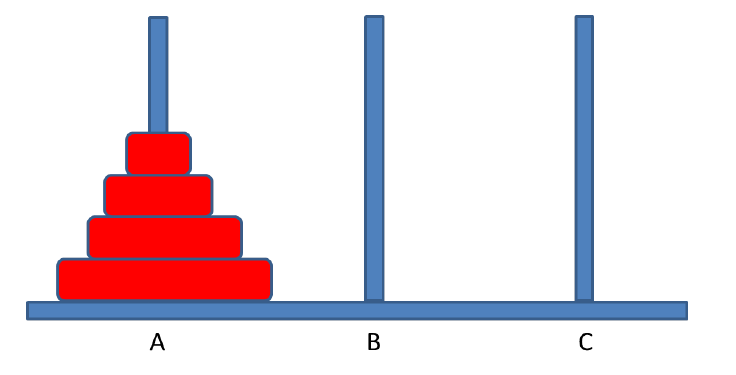
\includegraphics[width=12cm]{aufgabe-hanoi.png}
	\end{figure}
	\vspace{-20pt}
	\begin{lstlisting}
		# hanoi.py
		def hanoi(n, start, end, helper): 
			if n == 1:
			print(start + "->" + end)  
			else:
				hanoi(n-1, start, helper, end)
				print(start + "->" + end)
				hanoi(n-1, helper, end, start)
		
		def user_input():
			return int(input())
		
		if __name__ == "__main__": 
			n = user_input()
			hanoi(n, 'A', 'C', 'B') 
	\end{lstlisting}
\\
\textmd{
Da man für eine Scheibe einen Zug, für 2 Scheiben 3 Züge und für 3 Scheiben 7 Züge benötigt, 
lässt sich ein Pattern naheliegen, dass man allgemein für n Scheiben $2^n - 1$ Züge benötigt. 
}

	\begin{proof}
		\section*{\small Beweisen Sie induktiv, dass diese Formel richtig ist} 
		\vspace{-2mm}
		\textbf{Vollständige Induktion} \\
		[1mm]
		\textit{Induktionsanfang:} \\
		[1mm]
		Für \( n = 1 \) $\Rightarrow$  \( 2^1 - 1 = 1 \) $\longleftarrow$ ist wahr \\
		[1mm]
		\textit{Induktionsvoraussetzung:} \\
		[1mm]
		Gilt für jede \( n \in \mathbb{N} \) \\
		[1mm]
		\textit{Induktionsschritt:} \\
		[1mm]
		Für \( n = n + 1 \) $\Rightarrow$ \( 2^{n + 1} - 1 = 2 * 2^n - 1 = 2*(2^n - 1) \) $\longleftarrow$ Voraussetzung \\
	\end{proof}
	
		\section*{\small Es ist nicht möglich, den Turm mit weniger Zügen zu versetzen}
		\vspace{-2mm}
	\textit{Annahme:} Es ist möglich, den Turm von Hanoi mit weniger als \( 2^n - 1 \) Zügen zu versetzen.  
	 	\vspace{-5pt}
		\[
		n = 1 \quad \Rightarrow \quad 2^{n-1} - 1 = 2^{1-1} - 1 = 2^0 - 1 = 0.
		\]
		Da aber mindestens 1 Zug benötigt wird, folgt, $ \lightning $

    \section{Extra Aufgaben}
    
    \subsection{Aufgabe 3.10} 
Wir betrachten die folgende rekursiv definierte Folge:
$$b_{n} =
\begin{cases} 
    1, \text{für  } n = 1 \\
    \sqrt{1 + b_{n-1}}, \text{für  } n > 2

\end{cases}$$

\begin{proof}
Beweisen dass diese Folge gegen den goldenen Schnitt konvergiert:
$$
\lim{n \rightarrow \inf} b_{n} = \frac{1+ \sqrt{5}}{2}  
$$

\textbf{Antwort:} 
Um zu zeigen, dass die rekursiv definierte Folge $ b_n $ gegen den goldenen Schnitt $\phi = \frac{1 + \sqrt{5}}{2}$ konvergiert, betrachten wir die Definition der Folge:
$$
b_n = \begin{cases} 
1, & \text{für } n = 1 \\ 
\sqrt{1 + b_{n-1}}, & \text{für } n > 1 
\end{cases}
$$

\textbf{Schritt 1:} Zu Zeigen, dass die Folge beschränkt und monoton ist:

Zuerst zeigen wir, dass die Folge $ b_n$ beschränkt ist. Wir vermuten, dass $ b_n < \phi $ für alle $ n $. \\
Wir zeigen dies durch Induktion.

\textbf{Induktionsanfang:} Für $ n = 1$ haben wir $ b_1 = 1 < \phi $.$

\textbf{Induktionsannahme:} Angenommen, $ b_k < \phi $ für ein $ k \geq 1 .$

\textbf{Induktionsschritt:} Wir zeigen, dass $_{k+1} < \phi $:

$$
b_{k+1} = \sqrt{1 + b_k} < \sqrt{1 + \phi}
$$

Da $ \phi = \frac{1 + \sqrt{5}}{2} $, gilt:

$
\sqrt{1 + \phi} = \sqrt{1 + \frac{1 + \sqrt{5}}{2}} = \sqrt{\frac{3 + \sqrt{5}}{2}}
$
Nun zeigen wir, dass $\sqrt{\frac{3 + \sqrt{5}}{2}} < \phi $

$$
\phi^2 = \left(\frac{1 + \sqrt{5}}{2}\right)^2 = \frac{1 + 2\sqrt{5} + 5}{4} = \frac{6 + 2\sqrt{5}}{4} = \frac{3 + \sqrt{5}}{2}
$$

Somit ist $ \sqrt{1 + \phi} < \phi \Rightarrow b_{k+1} < \phi $.

Durch Induktion folgt, dass $ b_n < \phi $ für alle $ n $.


\textbf{Schritt 2:} Zu Zeigen, dass die Folge monoton wächst

Nun zeigen wir, dass $ b_n $ monoton wachsend ist, d.h. $ b_n < b_{n+1} \forall n $.
\\
Wir zeigen dies durch vollsändige Induktion:

\textbf{Induktionsanfang:} Für $n = 1$ haben wir $ b_1 = 1 < b_2 = \sqrt{1 + 1} = \sqrt{2} .$

\textbf{Induktionsannahme:} Angenommen, $ b_k < b_{k+1} $

\textbf{Induktionsschritt:} Wir zeigen, dass $b_{k+1} < b_{k+2} :$

$$
b_{k+2} = \sqrt{1 + b_{k+1}}
$$

Da $ b_k < b_{k+1} $, gilt $ 1 + b_k < 1 + b_{k+1} .$ 

Da die Funktion $(x) = \sqrt{1 + x}$ monoton wachsend ist, folgt: 

$$
b_{k+1} = \sqrt{1 + b_k} < \sqrt{1 + b_{k+1}} = b_{k+2}
$$

Somit ist $ b_n $ monoton wachsend.

Da $b_n$ eine monoton wachsende und beschränkte Folge ist, konvergiert sie. 

Sei $L = \lim_{n \to \infty} b_n $ dann gilt:

$$
L = \sqrt{1 + L}
$$

Quadrieren beider Seiten ergibt:

$$
L^2 = 1 + L \implies L^2 - L - 1 = 0
$$

%Die Lösungen dieser quadratischen Gleichung sind:

$$
=> L = \frac{1 \pm \sqrt{5}}{2}
$$

Da $ b_n >= 0$ %positiv ist, nehmen wir die positive Lösung:

$$
=> L = \frac{1 + \sqrt{5}}{2} = \phi
$$


%Wir haben gezeigt, dass die Folge $ b_n $ gegen den goldenen Schnitt konvergiert:

$$
=> \lim_{n \to \infty} b_n = \frac{1 + \sqrt{5}}{2}
$$
\end{proof}
%$\square$
    
    \href{https://github.com/SpiXFamily/Rekursion-MLL}{https://github.com/SpiXFamily/Rekursion-MLL}
  
        \centering
        
\includegraphics[width=0.5 \linewidth]{github-qr.png}
        %\caption{Caption}
        %\label{fig:enter-label}
  
\end{document}